\documentclass[11pt,letterpaper]{article}
\usepackage[utf8]{inputenc}
\usepackage[T1]{fontenc}
\usepackage{amsmath}
\usepackage[spanish,mexico]{babel}
\usepackage{mathpazo}              % Palatino para texto + matemáticas
\usepackage[margin=2.5cm]{geometry}
\usepackage{graphicx}
% Rutas múltiples: repo local (../Figures/) y zip plano de Overleaf (figures/).
\graphicspath{{../Figures/}{figures/}{Figures/}{./}}
\usepackage{booktabs}
\usepackage{xcolor}
\definecolor{uacjazul}{HTML}{003CA6}
\definecolor{uacjoro}{HTML}{C8962E}
\definecolor{uacjgris}{HTML}{555559}
\usepackage[colorlinks=true,linkcolor=uacjazul,citecolor=uacjazul,urlcolor=uacjazul]{hyperref}
\usepackage{fancyhdr}
\usepackage{titlesec}
\usepackage{caption}
\usepackage{siunitx}
% Formato mexicano: punto decimal, coma de miles, redondeo a 2 decimales.
% El bloque se define aquí y se RE-aplica en \AtBeginDocument para imponerse
% sobre el locale que babel-spanish fija al iniciar el documento.
\newcommand{\formatomexicano}{%
  \sisetup{
    input-decimal-markers = {.},
    output-decimal-marker = {.},
    group-separator       = {,},
    group-minimum-digits  = 4,
    round-mode            = places,
    round-precision       = 2,
  }%
}
\formatomexicano
\AtBeginDocument{\formatomexicano}
\usepackage{subcaption}
\usepackage{enumitem}

% --- Valores numéricos generados por el código (NO editar a mano) ---
% === ARCHIVO GENERADO AUTOMÁTICAMENTE por src/export_latex.py ===
% No editar a mano. Regenerar con: python -m src.main

\newcommand{\PostPondCosto}{20.1774}
\newcommand{\PostPondTiempo}{23.3165}
\newcommand{\PostLexCosto}{200.0}
\newcommand{\PostLexTiempo}{0.0}
\newcommand{\AprioriPondCosto}{17.9985}
\newcommand{\AprioriPondTiempo}{24.5009}
\newcommand{\AprioriPondVarUno}{1.4998}
\newcommand{\AprioriPondVarDos}{1.5001}
\newcommand{\AprioriLexCosto}{200.0}
\newcommand{\AprioriLexTiempo}{0.0}
\newcommand{\AprioriLexVarUno}{5.0}
\newcommand{\AprioriLexVarDos}{5.0}
\newcommand{\DiffPondCosto}{2.1789}
\newcommand{\DiffPondTiempo}{1.1844}
\newcommand{\MetHipervolumen}{8275.4031}
\newcommand{\MetSpacing}{0.9774}
\newcommand{\MetNSol}{100}
\newcommand{\MetMinFuno}{0.0}
\newcommand{\MetMaxFuno}{200.0}
\newcommand{\MetMinFdos}{0.0}
\newcommand{\MetMaxFdos}{50.0}
\newcommand{\MetSeed}{1}


% --- Encabezado / pie de página ---
\pagestyle{fancy}
\fancyhf{}
\fancyhead[L]{\small\textcolor{uacjazul}{MIAAD · Optimización Inteligente}}
\fancyhead[R]{\small\textcolor{uacjazul}{Análisis Multicriterio}}
\fancyfoot[C]{\thepage}
\renewcommand{\headrulewidth}{0.4pt}
\renewcommand{\headrule}{\hbox to\headwidth{\color{uacjazul}\leaders\hrule height \headrulewidth\hfill}}

% --- Estilo de secciones ---
\titleformat{\section}{\Large\bfseries\color{uacjazul}}{\thesection.}{0.6em}{}
\titleformat{\subsection}{\large\bfseries\color{uacjgris}}{\thesubsection}{0.6em}{}

\title{}
\date{}

\begin{document}

% ====================== PORTADA ======================
\begin{titlepage}
\thispagestyle{empty}
\centering
\vspace*{1.5cm}

{\color{uacjazul}\rule{\linewidth}{1.2pt}}\\[0.4cm]
{\color{uacjgris}\large Universidad Autónoma de Ciudad Juárez}\\[0.2cm]
{\color{uacjgris}\large Maestría en Ingeniería en Análisis y Administración de Datos (MIAAD)}\\[0.5cm]
{\color{uacjazul}\rule{\linewidth}{1.2pt}}\\[2.0cm]

{\Huge\bfseries\color{uacjazul} Análisis Comparativo de Estrategias de Decisión Multicriterio\par}
\vspace{0.4cm}
{\LARGE\color{uacjazul} A Priori vs. A Posteriori\par}
\vspace{0.8cm}
{\large\itshape Práctica de Laboratorio --- Optimización Inteligente\par}

\vspace{2.5cm}

\begin{tabular}{rl}
\textbf{Alumno:} & Javier Augusto Rebull Saucedo \\
\textbf{Matrícula:} & 263483 \\
\textbf{Profesor:} & Mtro. Raúl Gibrán Porras Alaniz \\
\textbf{Materia:} & Optimización Inteligente \\
\textbf{Programa:} & MIAAD --- UACJ \\
\textbf{Fecha:} & Mayo de 2026 \\
\end{tabular}

\vspace{1.2cm}

\begin{tabular}{rl}
\textbf{Repositorio:} & \href{https://github.com/jrebull/MIAAD_SMART_Multicriterio}{github.com/jrebull/MIAAD\_SMART\_Multicriterio} \\
\textbf{Dashboard:} & \href{https://multicriterio.streamlit.app}{multicriterio.streamlit.app} \\
\end{tabular}

\vfill
{\color{uacjoro}\rule{\linewidth}{2pt}}\\[0.3cm]
{\small\color{uacjgris} Reporte reproducible --- todos los valores numéricos provienen de
\texttt{results/selected\_solutions.json} y \texttt{results/metrics.json}\par}
\end{titlepage}

% ====================== ÍNDICE ======================
\tableofcontents
\newpage

% ====================== SECCIONES ======================
\section{Introducción}

En la optimización del mundo real rara vez existe un único criterio de éxito.
El presente trabajo analiza un problema \textbf{bi-objetivo} en conflicto,
inspirado en una decisión logística de ruteo, donde se busca simultáneamente
\emph{minimizar} dos magnitudes que se contraponen:

\begin{itemize}[noitemsep]
  \item $f_1$: \textbf{Costo Operativo} de la operación.
  \item $f_2$: \textbf{Tiempo de Entrega} al cliente.
\end{itemize}

El objetivo pedagógico no es únicamente resolver el problema, sino comprender
cómo el \textbf{momento} en que el tomador de decisiones expresa sus
preferencias altera el resultado final. Contrastamos dos filosofías
metodológicas~\cite{miettinen1999nonlinear,marler2004survey}:

\begin{itemize}[noitemsep]
  \item \textbf{A Posteriori}: primero se aproxima \emph{todo} el frente de
        Pareto (con NSGA-II~\cite{deb2002nsga2}) y, sólo después, el decisor
        elige una solución sobre el conjunto no dominado.
  \item \textbf{A Priori}: el decisor inyecta sus preferencias
        \emph{antes} de optimizar, colapsando el problema bi-objetivo a uno
        mono-objetivo que se resuelve con un Algoritmo Genético (GA) clásico.
\end{itemize}

\subsection{Formulación matemática}

El problema continuo, denominado \texttt{RoutingProxyProblem}, se define sobre
el dominio $\mathbf{x} = (x_1, x_2) \in [0, 5]^2$ como:

\begin{align}
  \min_{\mathbf{x}} \quad & f_1(\mathbf{x}) = 4x_1^2 + 4x_2^2 \\
  \min_{\mathbf{x}} \quad & f_2(\mathbf{x}) = (x_1 - 5)^2 + (x_2 - 5)^2 \\
  \text{s.a.} \quad & 0 \le x_1, x_2 \le 5 . \nonumber
\end{align}

La tensión es geométrica e intuitiva: $f_1$ se minimiza en el origen
$\mathbf{x}=(0,0)$, mientras que $f_2$ se minimiza en la esquina opuesta
$\mathbf{x}=(5,5)$. Ninguna solución puede satisfacer ambos óptimos a la vez,
lo que da lugar a un frente de Pareto convexo de soluciones de compromiso.

\subsection{Objetivos del reporte}

Este documento responde explícitamente a cuatro preguntas: (1) la
visualización conjunta de las estrategias; (2) si la \emph{suma ponderada}
a priori coincide con su análoga a posteriori; (3) qué ocurre con $f_1$ al
aplicar un criterio \emph{lexicográfico} estricto sobre $f_2$; y (4) una
recomendación profesional sobre cuándo conviene cada enfoque. Todo el análisis
es \textbf{reproducible} con semilla fija (\texttt{seed = \MetSeed}).

\section{Metodología}

Se implementaron en Python (módulo \texttt{src/}) las dos estrategias de
decisión sobre el mismo problema bi-objetivo, garantizando reproducibilidad
bit-a-bit mediante una semilla fija en cada llamada a \texttt{minimize()}.

\subsection{Estrategia A Posteriori: NSGA-II + post-selección}

Se aproxima el frente de Pareto completo con el algoritmo
NSGA-II~\cite{deb2002nsga2,blank2020pymoo}. Sobre el conjunto de \MetNSol{}
soluciones no dominadas resultantes, el tomador de decisiones aplica dos
criterios de selección \emph{a posteriori}:

\begin{itemize}[noitemsep]
  \item \textbf{Suma ponderada normalizada.} Se normaliza cada objetivo al
        rango $[0,1]$ usando los extremos del frente y se minimiza la
        combinación $0.7\,\tilde{f_1} + 0.3\,\tilde{f_2}$, otorgando 70\,\% de
        importancia al costo y 30\,\% al tiempo.
  \item \textbf{Lexicográfica.} Se prioriza estrictamente el Tiempo ($f_2$):
        se elige la solución del frente con menor $f_2$.
\end{itemize}

\subsection{Estrategia A Priori: GA mono-objetivo}

Aquí las preferencias se inyectan \emph{antes} de optimizar, transformando el
problema en mono-objetivo y resolviéndolo con un GA clásico:

\begin{itemize}[noitemsep]
  \item \textbf{Suma ponderada directa.} Con un \emph{escalamiento manual}
        aproximado a los rangos de cada objetivo, se minimiza
        \[
          g(\mathbf{x}) = 0.7 \cdot \frac{f_1(\mathbf{x})}{200}
                        + 0.3 \cdot \frac{f_2(\mathbf{x})}{50}.
        \]
  \item \textbf{Lexicográfica directa.} Se optimiza únicamente el objetivo
        prioritario, $f_2$, ignorando por completo a $f_1$ durante la búsqueda.
\end{itemize}

\subsection{Parámetros de ejecución}

La Tabla~\ref{tab:parametros} resume la configuración. Ambos algoritmos usan el
mismo tamaño de población y número de generaciones para una comparación justa.

\begin{table}[h]
  \centering
  \caption{Parámetros de los algoritmos evolutivos.}
  \label{tab:parametros}
  \begin{tabular}{lll}
    \toprule
    \textbf{Parámetro} & \textbf{A Posteriori (NSGA-II)} & \textbf{A Priori (GA)} \\
    \midrule
    Tamaño de población & \num{100} & \num{100} \\
    Generaciones        & \num{100} & \num{100} \\
    Semilla             & \MetSeed & \MetSeed \\
    Objetivos           & 2 ($f_1, f_2$) & 1 (escalar) \\
    Pesos $(w_1, w_2)$  & $(0.7,\ 0.3)$ & $(0.7,\ 0.3)$ \\
    Escalamiento        & normalización por rango & manual ($f_1/200,\ f_2/50$) \\
    \bottomrule
  \end{tabular}
\end{table}

\subsection{Métricas de calidad del frente}

Para caracterizar el frente NSGA-II se reportan: el \textbf{hipervolumen}
(volumen dominado respecto al punto de referencia $(\num{200}, \num{50})$),
indicador de convergencia y diversidad; y el \textbf{spacing} de
Schott~\cite{coello2007evolutionary}, que mide la uniformidad de la
distribución de soluciones a lo largo del frente.

\section{Resultados}

\subsection{Visualización conjunta de las estrategias}

La Figura~\ref{fig:scatter} presenta el frente de Pareto aproximado por
NSGA-II (círculos azules) junto con las cuatro soluciones seleccionadas por
las distintas estrategias. Esta gráfica responde al \textbf{primer entregable}
del enunciado: la comparación espacial de las decisiones con la leyenda
visible. El frente puede explorarse de forma interactiva (moviendo los pesos y
el criterio lexicográfico) en el dashboard publicado en
\href{https://multicriterio.streamlit.app}{multicriterio.streamlit.app}.

\begin{figure}[h]
  \centering
  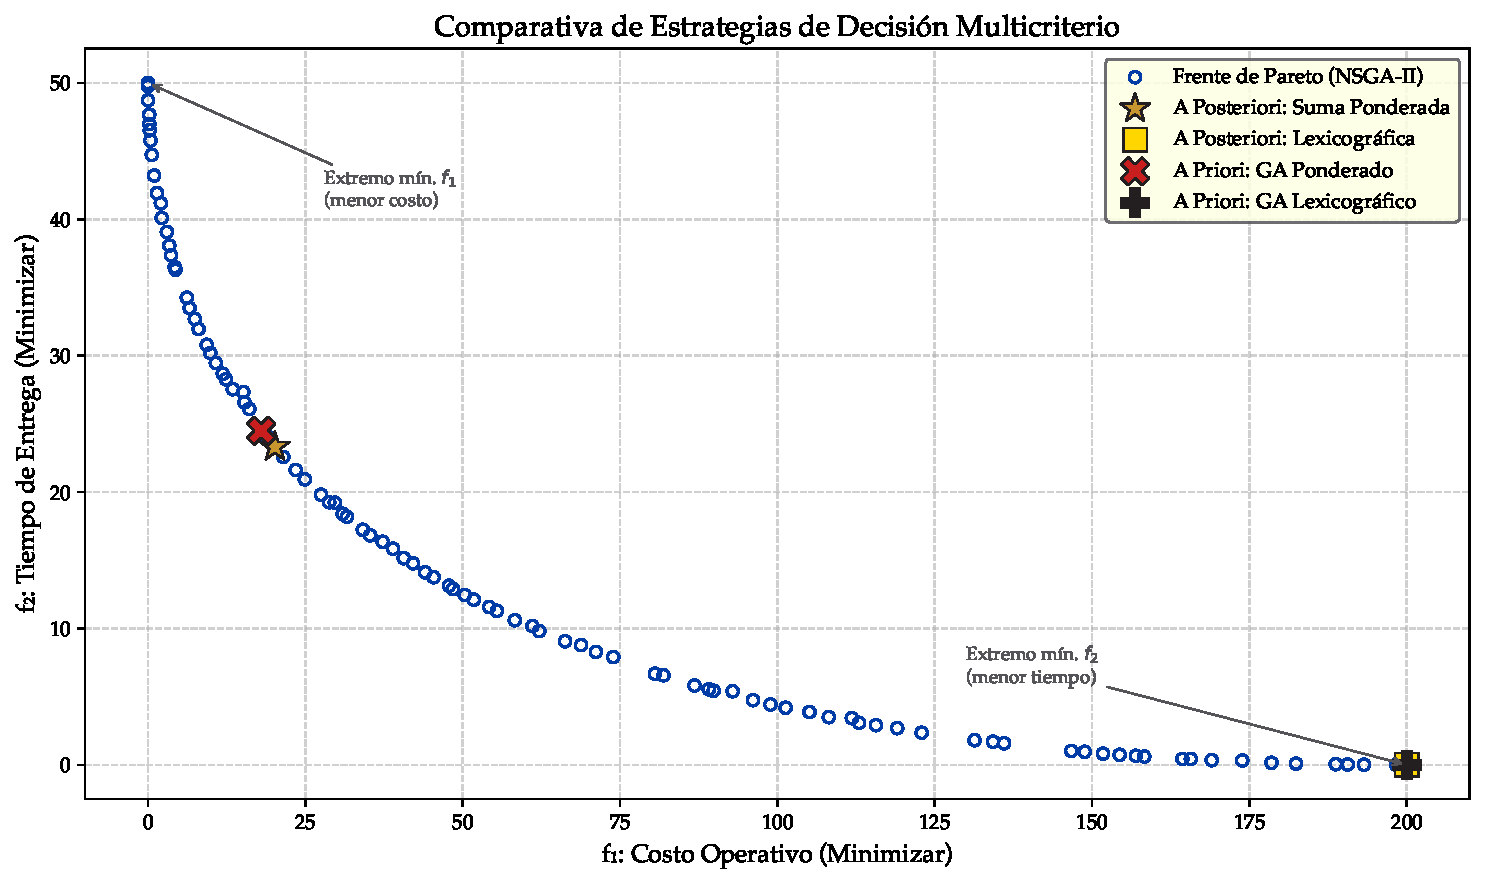
\includegraphics[width=\linewidth]{scatter_estrategias.pdf}
  \caption{Comparativa de estrategias de decisión multicriterio. El frente de
  Pareto (NSGA-II) define la curva de soluciones de compromiso. Las dos
  soluciones \emph{ponderadas} (a priori y a posteriori) caen prácticamente
  superpuestas en el ``codo'' del frente, mientras que ambas soluciones
  \emph{lexicográficas} coinciden en el extremo de menor tiempo
  $(f_1, f_2) \approx (\num{200}, \num{0})$.}
  \label{fig:scatter}
\end{figure}

\subsection{Soluciones seleccionadas}

La Tabla~\ref{tab:soluciones} reporta las cuatro soluciones. Todos los valores
se leen directamente de \texttt{results/\allowbreak selected\_solutions.json}.

\begin{table}[h]
  \centering
  \caption{Soluciones obtenidas por cada estrategia de decisión.}
  \label{tab:soluciones}
  \begin{tabular}{llSS}
    \toprule
    \textbf{Enfoque} & \textbf{Criterio} & {\textbf{$f_1$ (Costo)}} & {\textbf{$f_2$ (Tiempo)}} \\
    \midrule
    A Posteriori & Suma Ponderada  & \PostPondCosto    & \PostPondTiempo \\
    A Posteriori & Lexicográfica   & \PostLexCosto     & \PostLexTiempo \\
    A Priori     & GA Ponderado    & \AprioriPondCosto & \AprioriPondTiempo \\
    A Priori     & GA Lexicográfico& \AprioriLexCosto  & \AprioriLexTiempo \\
    \bottomrule
  \end{tabular}
\end{table}

\subsection{Calidad del frente de Pareto}

El frente aproximado por NSGA-II consta de \MetNSol{} soluciones no dominadas,
con los siguientes indicadores (de \texttt{results/metrics.json}):

\begin{itemize}[noitemsep]
  \item \textbf{Hipervolumen} (ref.\ $(\num{200},\num{50})$):
        \num{\MetHipervolumen}.
  \item \textbf{Spacing} de Schott: \num{\MetSpacing} (valor bajo $\Rightarrow$
        distribución uniforme).
  \item \textbf{Extremos del frente:} $f_1 \in [\num{\MetMinFuno},\ \num{\MetMaxFuno}]$,
        $f_2 \in [\num{\MetMinFdos},\ \num{\MetMaxFdos}]$.
\end{itemize}

Los extremos coinciden exactamente con la predicción analítica: el frente va
de $(\num{0}, \num{50})$, correspondiente a $\mathbf{x}=(0,0)$ (mínimo costo),
hasta $(\num{200}, \num{0})$, correspondiente a $\mathbf{x}=(5,5)$ (mínimo
tiempo). Esta concordancia valida numéricamente la implementación.

\section{Análisis de la Suma Ponderada (Pregunta 2)}

\textit{¿Existe una diferencia significativa entre la solución encontrada
calculando los pesos a priori con el GA frente a seleccionarla a posteriori
del frente de Pareto generado por NSGA-II? Explica por qué coinciden o
difieren.}

\subsection{Comparación cuantitativa}

\begin{table}[h]
  \centering
  \caption{Suma ponderada: A Priori (GA) vs.\ A Posteriori (NSGA-II).}
  \label{tab:ponderada}
  \begin{tabular}{lSSS}
    \toprule
    & {\textbf{$f_1$ (Costo)}} & {\textbf{$f_2$ (Tiempo)}} & {\textbf{Suma escalada}} \\
    \midrule
    A Priori (GA)        & \AprioriPondCosto & \AprioriPondTiempo & {---} \\
    A Posteriori (NSGA-II)& \PostPondCosto   & \PostPondTiempo    & {---} \\
    \midrule
    Diferencia absoluta  & \DiffPondCosto    & \DiffPondTiempo    & {---} \\
    \bottomrule
  \end{tabular}
\end{table}

Las dos soluciones son \textbf{muy cercanas pero no idénticas}: difieren en
apenas $\num{\DiffPondCosto}$ unidades de costo y $\num{\DiffPondTiempo}$
unidades de tiempo. En la Figura~\ref{fig:scatter} ambos marcadores (estrella
oro y equis roja) caen prácticamente superpuestos sobre el ``codo'' del frente.

\subsection{Por qué coinciden}

La razón es geométrica. El método de suma ponderada equivale a buscar la
solución que toca primero una recta de pendiente $-w_1/w_2$ que barre el
espacio de objetivos. Cuando el frente de Pareto es \textbf{convexo} ---como
ocurre aquí--- esa recta toca el frente en un único punto bien definido, y
\emph{cualquier} método que minimice la misma combinación lineal converge
esencialmente al mismo lugar~\cite{marler2004survey,miettinen1999nonlinear}.
Por construcción, el problema $f_1 = 4(x_1^2+x_2^2)$, $f_2 = (x_1-5)^2+(x_2-5)^2$
genera un frente convexo, lo que explica la coincidencia.

De hecho, la solución A Priori converge a $\mathbf{x} \approx
(\num{\AprioriPondVarUno}, \num{\AprioriPondVarDos})$, que coincide con el
óptimo analítico exacto $(1.5, 1.5)$ obtenible por simetría e igualación de
derivadas. El GA recuperó el óptimo teórico sin error apreciable.

\subsection{Por qué difieren levemente}

La pequeña discrepancia se debe a que \textbf{ambos enfoques no minimizan
exactamente la misma función escalar}:

\begin{itemize}[noitemsep]
  \item El A Priori usa un \textbf{escalamiento manual fijo} ($f_1/200$,
        $f_2/50$), denominadores elegidos a ojo según los rangos esperados.
  \item El A Posteriori \textbf{normaliza por los extremos reales} del frente
        muestreado, que dependen de las \MetNSol{} soluciones encontradas.
\end{itemize}

Como los factores de escala difieren, la dirección de preferencia efectiva se
inclina ligeramente distinto, desplazando el punto seleccionado unas pocas
unidades. Además, el A Posteriori sólo puede elegir entre los puntos
\emph{discretos} del frente muestreado, no sobre el continuo. En resumen: no
hay diferencia \emph{significativa} ---el sesgo del escalamiento manual es
marginal cuando el frente es convexo--- pero sí una diferencia \emph{medible}
y explicable.

\section{Análisis Lexicográfico (Pregunta 3)}

\textit{Al aplicar la estrategia lexicográfica directa minimizando sólo $f_2$,
¿qué sucedió con el valor de $f_1$? Compara este valor con el extremo del
frente de Pareto de NSGA-II.}

\subsection{Qué le ocurrió a $f_1$}

Al optimizar \emph{exclusivamente} el Tiempo ($f_2$), el GA llevó la solución
a $\mathbf{x} = (\num{\AprioriLexVarUno}, \num{\AprioriLexVarDos})$, donde
$f_2$ alcanza su mínimo global $\num{\AprioriLexTiempo}$. Pero al ignorar por
completo al Costo, éste se disparó hasta su \textbf{valor máximo posible} en
el dominio:
\[
  f_1 = \num{\AprioriLexCosto}, \qquad f_2 = \num{\AprioriLexTiempo}.
\]
Esto es exactamente lo que predice la teoría: minimizar $f_2 = (x_1-5)^2 +
(x_2-5)^2$ empuja la solución a la esquina $(5,5)$, que es justamente el punto
donde $f_1 = 4(25)+4(25) = \num{200}$ es \emph{máximo}. La prioridad rígida
sobre un objetivo sacrifica por completo al otro.

\subsection{Comparación con el extremo del frente NSGA-II}

El frente aproximado por NSGA-II tiene su extremo de menor tiempo en
$f_1 = \num{\MetMaxFuno}$, $f_2 = \num{\MetMinFdos}$ (la solución
\texttt{post\_lexico} de la Tabla~\ref{tab:soluciones}). Como se aprecia en la
Figura~\ref{fig:zoom}, \textbf{ambos enfoques lexicográficos aterrizan en el
mismo punto} $(\num{200}, \num{0})$: la decisión lexicográfica a priori y la
selección lexicográfica a posteriori son indistinguibles aquí, porque ambas
persiguen el mismo objetivo extremo del frente.

\begin{figure}[h]
  \centering
  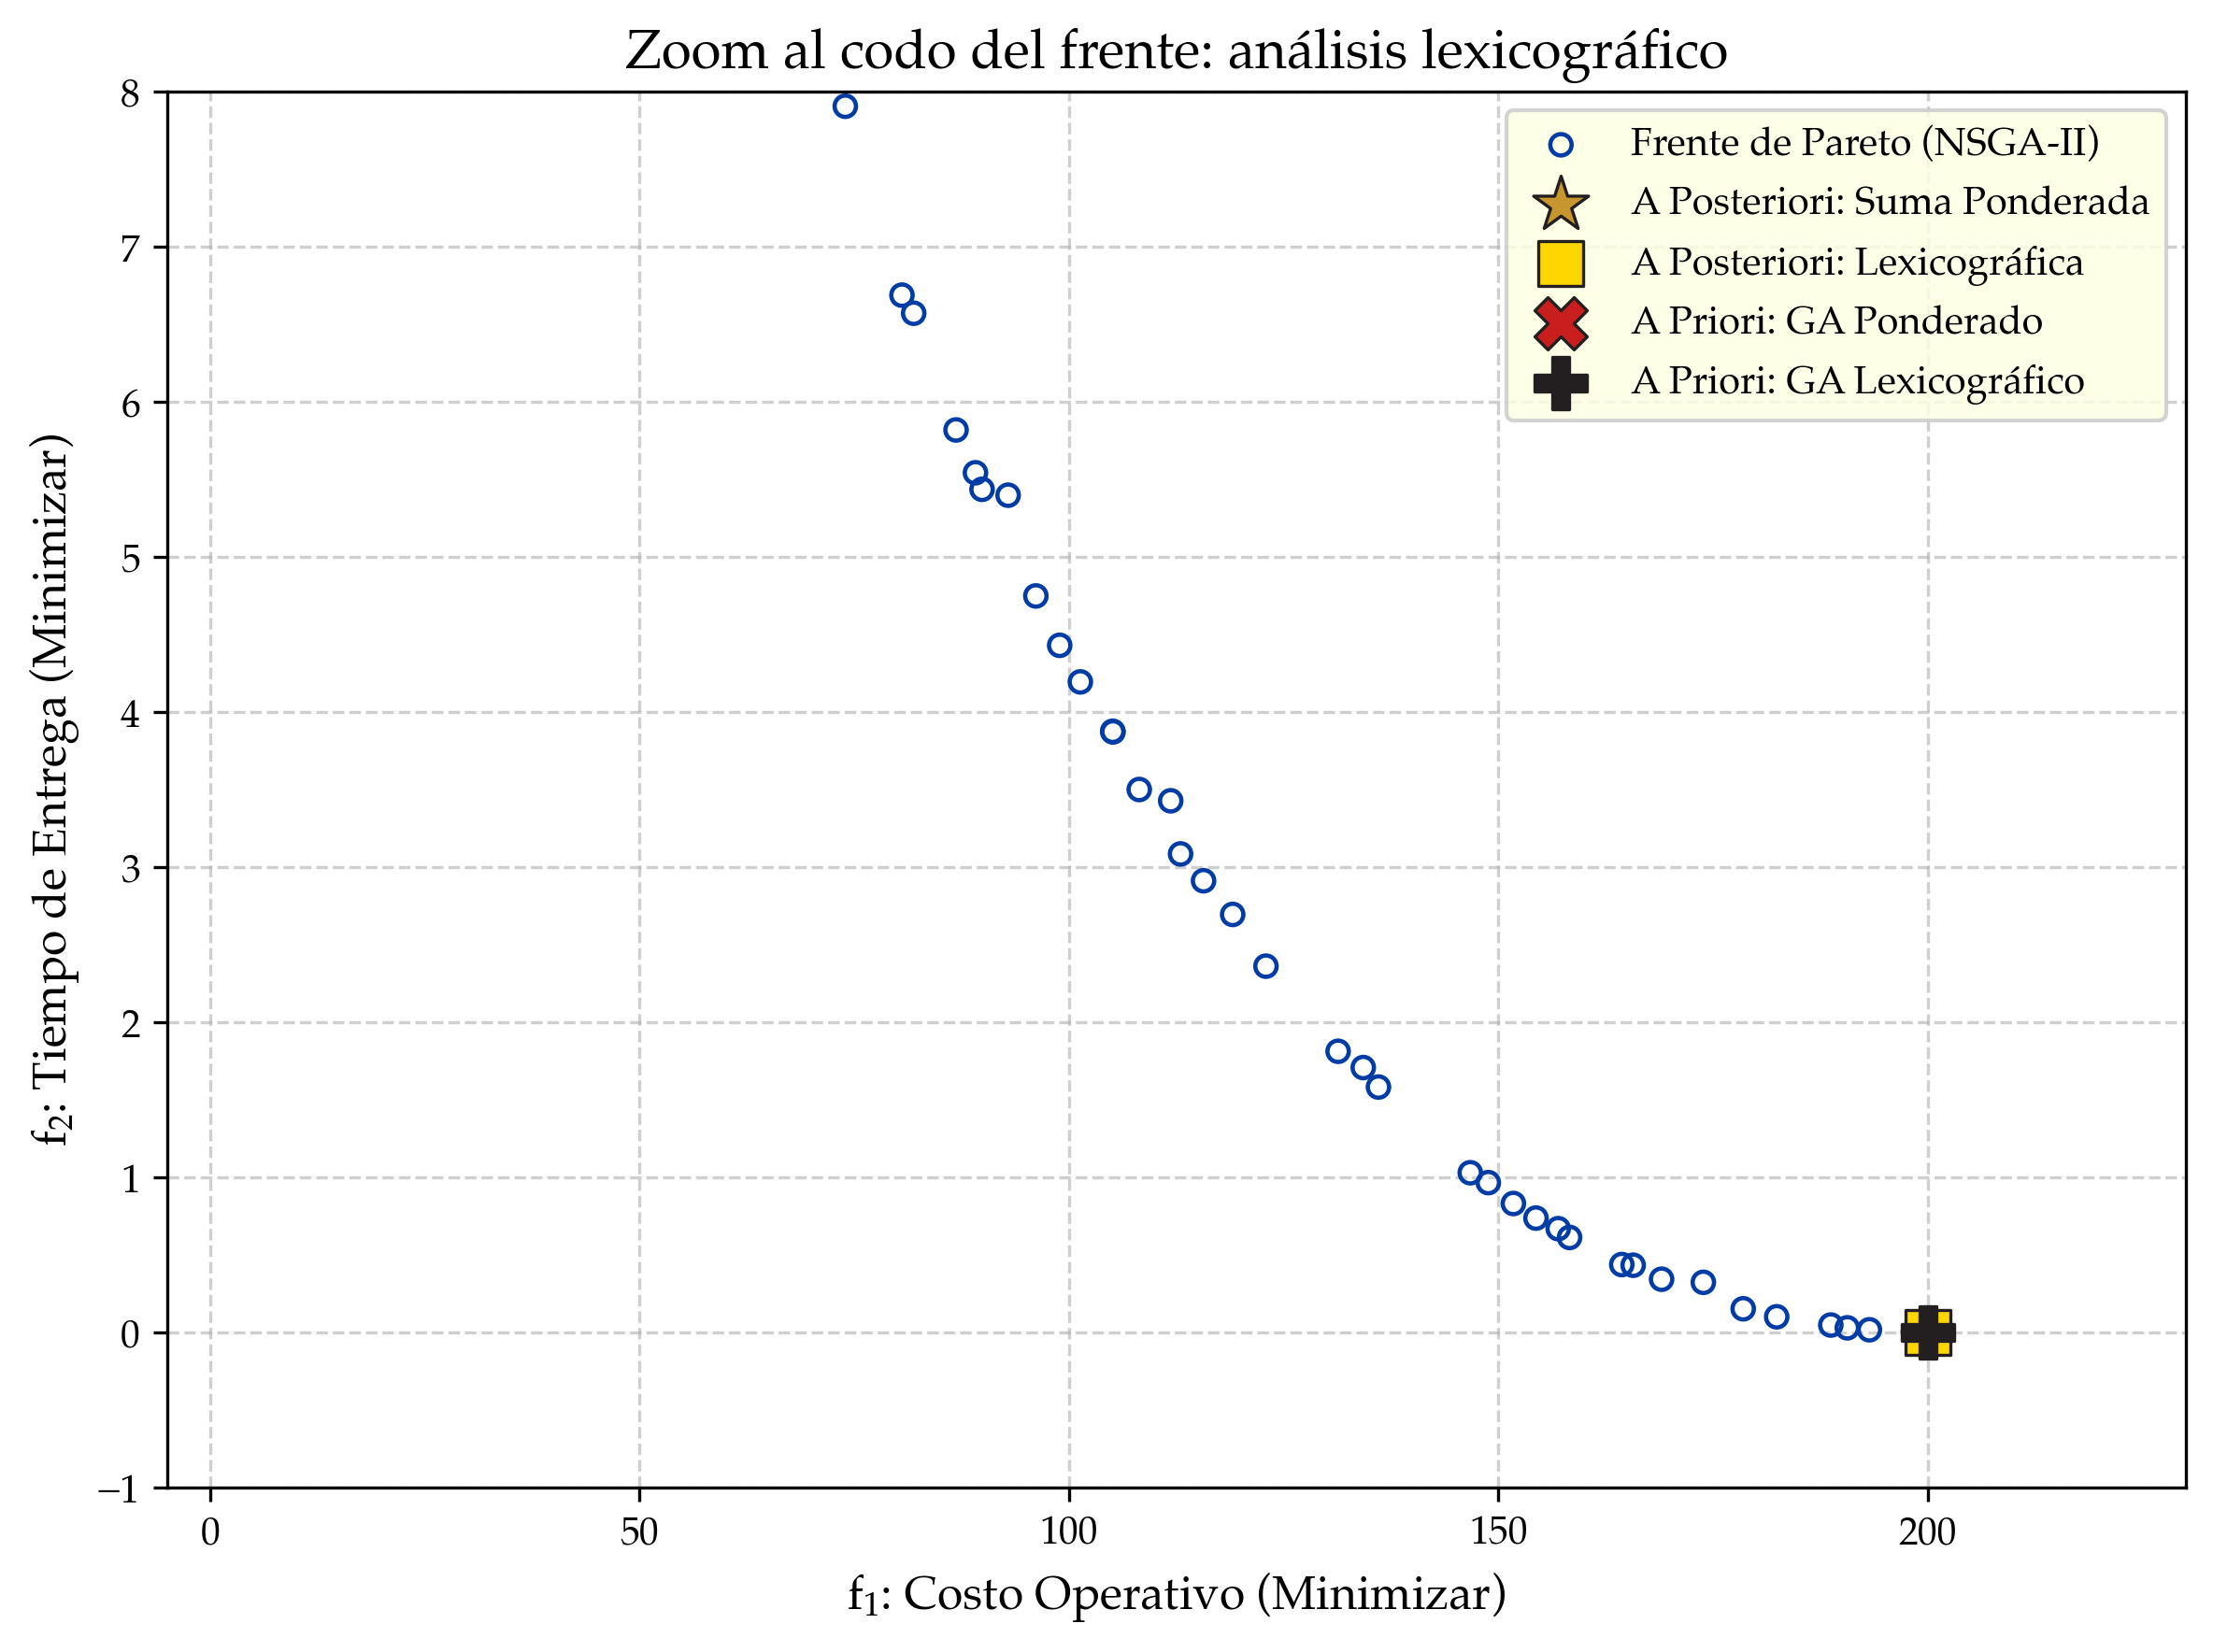
\includegraphics[width=0.85\linewidth]{pareto_front_zoom.png}
  \caption{Zoom al codo del frente. Las soluciones lexicográficas (cuadrado
  amarillo y marcador negro) coinciden en el extremo $(\num{200}, \num{0})$,
  el punto de mayor costo del frente.}
  \label{fig:zoom}
\end{figure}

\subsection{El costo de la prioridad rígida}

La lección es contundente: pasar de la solución \emph{ponderada}
($f_1 \approx \num{\AprioriPondCosto}$) a la \emph{lexicográfica}
($f_1 = \num{\AprioriLexCosto}$) implica multiplicar el costo operativo por un
factor superior a $\times 10$ a cambio de recortar el tiempo desde
$\approx \num{\AprioriPondTiempo}$ hasta $\num{\AprioriLexTiempo}$. El enfoque
lexicográfico es apropiado únicamente cuando el objetivo prioritario es
verdaderamente \textbf{innegociable} (p.\ ej.\ una restricción regulatoria o
de seguridad); de lo contrario, ignora compromisos intermedios mucho más
eficientes que sí captura el frente de Pareto.

\section{Conclusión Profesional (Pregunta 4)}

\textit{Si fueras el ingeniero consultor de una empresa logística, ¿en qué
situación recomendarías invertir tiempo computacional en NSGA-II para mostrar
el frente completo, y en qué situación usarías un enfoque directo a priori?}

\subsection{El criterio de decisión: ¿conoces tus pesos?}

La pregunta no es ``¿qué algoritmo es mejor?'', sino ``¿qué tan seguro está el
negocio de sus preferencias \emph{antes} de optimizar?''. Mi experiencia en
banca (Santander US) lo ilustra con dos analogías directas:

\paragraph{Caso A --- Decisión estratégica única (recomiendo NSGA-II).}
Es análogo a definir la estrategia de \textbf{reabastecimiento de cajeros
(ATMs)}: el costo logístico del traslado de efectivo contra el SLA de
disponibilidad ante el cliente. Cuando la decisión es de alto impacto, se toma
una sola vez, involucra a múltiples \emph{stakeholders} (Operaciones, Riesgo,
Experiencia del Cliente) y \textbf{nadie tiene pesos claros consensuados},
vale la pena invertir el cómputo de NSGA-II. Mostrar el frente de Pareto
completo convierte una discusión política (``¿cuánto vale un minuto de
disponibilidad?'') en una negociación informada sobre compromisos concretos y
visibles. El frente es una herramienta de \emph{alineación organizacional},
no sólo de optimización.

\paragraph{Caso B --- Decisión operativa recurrente (recomiendo A Priori).}
Es análogo a la \textbf{asignación automática de líneas de crédito} o al
ruteo diario de reabastecimiento: decisiones que se ejecutan miles de veces,
con pesos ya \emph{aprendidos y estables} (el negocio sabe que prioriza, por
ejemplo, 70\,\% costo / 30\,\% tiempo). Aquí desplegar NSGA-II en cada corrida
sería un desperdicio: el enfoque a priori entrega en una fracción del tiempo
una solución que ---como demostró la Sección 4--- es prácticamente idéntica a
la que se elegiría sobre el frente completo, gracias a la convexidad del
problema.

\subsection{Síntesis de hallazgos}

\begin{itemize}[noitemsep]
  \item \textbf{Suma ponderada:} a priori y a posteriori \emph{convergen}
        (diferencia de sólo $\num{\DiffPondCosto}$ en costo) cuando el frente
        es convexo. El cómputo extra de NSGA-II no cambia la decisión.
  \item \textbf{Lexicográfica:} la prioridad rígida sobre $f_2$ disparó el
        costo a $f_1 = \num{\AprioriLexCosto}$ (el peor del frente). Útil sólo
        ante objetivos innegociables.
  \item \textbf{Valor del frente:} su retorno no es numérico sino de
        \emph{transparencia}: expone el menú completo de compromisos.
\end{itemize}

\subsection{Recomendación final}

\begin{center}
\fbox{\begin{minipage}{0.92\linewidth}
\textbf{Regla práctica.} Usa \textbf{A Posteriori (NSGA-II)} cuando la decisión
sea estratégica, única, con \emph{stakeholders} múltiples y sin pesos
consensuados: el frente alinea a la organización. Usa \textbf{A Priori (GA)}
cuando la decisión sea operativa, recurrente y con preferencias estables ya
conocidas: es más barato y, sobre frentes convexos, igual de acertado.
\end{minipage}}
\end{center}

En definitiva, el momento de expresar las preferencias debe alinearse con la
\textbf{naturaleza de la decisión}, no con la sofisticación del algoritmo
disponible. Un buen consultor elige la herramienta proporcional al problema.


% ====================== BIBLIOGRAFÍA ======================
\newpage
\bibliographystyle{plain}
\bibliography{references}

\end{document}
